\section{Cells}

Let us first introduce a discrete version of 2-dimensional space. Two-dimensional space supports geometric structures with either zero, one, or two dimensions: vertices, edges, and planes. These $k$-dimensional geometric structures are formally called $k$-cells for $k = 0, 1, 2$, represented by $\sigma^{(k)}$, where $k$ denotes the dimension of the cell. Three examples of $k$-cells are shown in Figure \ref{fig:cells}.
\begin{figure}[ht]
    \newsavebox\boxCell
    \savebox{\boxCell}{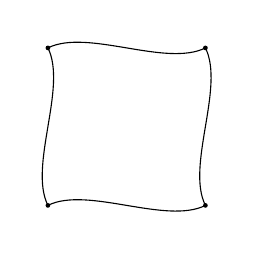
\begin{tikzpicture}
        \fill (0,0) circle (0.03);
        \fill (2,0) circle (0.03);
        \fill (2,2) circle (0.03);
        \fill (0,2) circle (0.03);
        \draw (0,0) .. controls (0.5,0.25) and (1.5,-0.25) .. (2,0) .. controls (1.75,0.5) and (2.25,1.5) .. (2,2) .. controls (1.5,1.75) and (0.5,2.25) .. (0,2) .. controls (0.25,1.5) and (-0.25,0.5) .. (0,0);
    \end{tikzpicture}}
    \centering
    \begin{subfigure}[c]{0.3\textwidth}
        \centering
        \vbox to \ht\boxCell{
            \vfill
            \begin{tikzpicture}
                \fill (1,1) circle (0.03);
            \end{tikzpicture}
            \vfill
        }
        \caption{0-cell (vertex)}
    \end{subfigure}
    \begin{subfigure}[c]{0.3\textwidth}
        \centering
        \vbox to \ht\boxCell{
            \vfill
            \begin{tikzpicture}
                \fill (0,1) circle (0.03);
                \draw (0,1) .. controls (0.5,1.25) and (1.5,0.75) .. (2,1);
                \fill (2,1) circle (0.03);
            \end{tikzpicture}
            \vfill
        }
        \caption{1-cell (edge)}
    \end{subfigure}
    \begin{subfigure}[c]{0.3\textwidth}
        \centering
        \usebox{\boxCell}
        \caption{2-cell (plane)}
        \label{fig:2cell}
    \end{subfigure}
    \caption{Examples of $k$-cells in two-dimensional space.}
    \label{fig:cells}
\end{figure}

A vertex is a 0-cell, an edge is a 1-cell, and a plane is a 2-cell. Just like a 1-cell is an edge with a length but with no position, a 2-cell can be thought of as a plane with an area, but no position. Notice that $k$-cells are bounded by $(k-1)$-cells and that a cell's shape is arbitrary, as indicated by the wavy edges. (\textit{Note:} The boundary of a 0-cell is empty by definition.)

We will be using vertices, edges, and planes as building blocks for our mesh. A mesh is a set of cells, called a cell-complex if the boundary of each cell is also part of the set. For example, the (rather primitive) mesh in Figure \ref{fig:2cell} is a cell-complex because the plane is bounded by edges and the edges are in turn bounded by vertices, all of which are part of the mesh.

\section{Chains and Cochains}

A set of $k$-cells is called a chain, written as
\begin{equation}
    \mathbf{c}^{(k)} = \{c_1 \sigma^{(k)}_1, \ldots, c_N \sigma^{(k)}_N \}
\end{equation}
where $N$ denotes the number of $k$-cells in the cell complex and $c_i$ denotes a weight $\in \mathbb{R}$. Chains merely differ by their weights, because all chains are composed of the same $k$-cells. The summation and multiplication of two $k$-chains is well-defined; in the case of summation, the weights add, and in the case of multiplication by a real number, the weights are multiplied by that real number. Thus, the set of $k$-chains, denoted $C^{(k)}$, is a linear vector space and the $k$-cells represent a basis for this vector space. Because $k$-cells represent a basis for $C^{(k)}$, we can define linear functionals that assign a value to $k$-cells. These linear functionals are called $k$-cochains and the set of all $k$-cochains is itself a linear vector space.

Let us briefly forget about those nitty mathematical details and reiterate the most important point: a chain is nothing more and nothing less than a set of cells and a cochain is essentially a set of cells tagged with a numerical value. Cochains are in practice realized as a vector of single or double precision numbers and it may help to think of cochains as such.

\section{Orientation}

In addition to dimension, $k$-cells have a property called orientation. A $k$-cell either has a positive or a negative orientation that can be freely defined on a per-cell basis, as long as the orientation remains unchanged thereafter. 

Figure \ref{fig:innerExample} shows three $k$-cells in two-dimensional space with an intrinsic orientation that we call inner-oriented $k$-cells. Inner-oriented vertices for instance, can either represent sources or sinks and are arbitrarily chosen to be source-like by default, as indicated by the outward pointing arrows in Figure \ref{fig:inner0Cell}. That it, an outflow is positive. Inner-oriented edges have a positive orientation when pointing to the right, as indicated by the arrows in Figure \ref{fig:inner1Cell}. It is somewhat awkward to think of the orientation of a plane, but an inner-oriented plane is defined positive when it is oriented counterclockwise, as indicated in Figure \ref{fig:inner2Cell}.

The simplices of our mesh are vertices, edges, and planes; their circumcentric counterparts are dual cells, composed of dual faces, dual edges, and dual vertices. Thus, all inner-oriented $k$-cells have an outer-oriented counterpart where its orientation is defined around or through the $k$-cell, rather than within. For example, an inner-oriented plane has a counterclockwise orientation whereas an outer-oriented plane represents a source. Figure \ref{fig:outerExample} shows three outer-oriented $k$-cells in two-dimensional space.
\begin{figure}[ht]
    \newsavebox\boxInner
    \savebox{\boxInner}{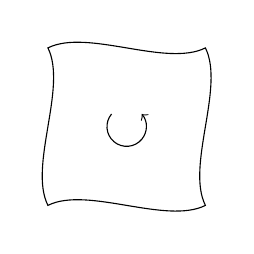
\begin{tikzpicture}
        \draw (0,0) .. controls (0.5,0.25) and (1.5,-0.25) .. (2,0) .. controls (1.75,0.5) and (2.25,1.5) .. (2,2) .. controls (1.5,1.75) and (0.5,2.25) .. (0,2) .. controls (0.25,1.5) and (-0.25,0.5) .. (0,0) -- cycle;
        \draw [->] (1,1) ++(140:0.25) arc (-220:40:0.25);
    \end{tikzpicture}}
    \centering
    \begin{subfigure}[c]{0.3\textwidth}
        \centering
        \vbox to \ht\boxInner{
            \vfill
            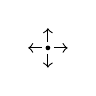
\begin{tikzpicture}
                \fill (1,1) circle (0.03);
                \draw [->] (1,1.075) -- (1,1.25);
                \draw [->] (1.075,1) -- (1.25,1);
                \draw [->] (1,0.925) -- (1,0.75);
                \draw [->] (0.925,1) -- (0.75,1);
            \end{tikzpicture}
            \vfill
        }
        \caption{0-cell}
        \label{fig:inner0Cell}
    \end{subfigure}
    \begin{subfigure}[c]{0.3\textwidth}
        \centering
        \vbox to \ht\boxInner{
            \vfill
            \begin{tikzpicture}
                \draw (0,1) .. controls (0.5,1.25) and (1.5,0.75) .. (2,1);
                \draw [->] (0.95,1.008) -- (1.05,0.992);
            \end{tikzpicture}
            \vfill
        }
        \caption{1-cell}
        \label{fig:inner1Cell}
    \end{subfigure}
    \begin{subfigure}[c]{0.3\textwidth}
        \centering
        \centering
        \usebox{\boxInner}
        \caption{2-cell}
        \label{fig:inner2Cell}
    \end{subfigure}
    \caption{Inner-oriented $k$-cells in two-dimensional space.}
    \label{fig:innerExample}
\end{figure}
\begin{figure}[ht]
    \newsavebox\outerBox
    \savebox{\outerBox}{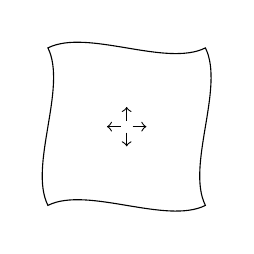
\begin{tikzpicture}
        \draw (0,0) .. controls (0.5,0.25) and (1.5,-0.25) .. (2,0) .. controls (1.75,0.5) and (2.25,1.5) .. (2,2) .. controls (1.5,1.75) and (0.5,2.25) .. (0,2) .. controls (0.25,1.5) and (-0.25,0.5) .. (0,0) -- cycle;
        \draw [->] (1,1.075) -- (1,1.25);
        \draw [->] (1.075,1) -- (1.25,1);
        \draw [->] (1,0.925) -- (1,0.75);
        \draw [->] (0.925,1) -- (0.75,1);
    \end{tikzpicture}}
    \centering
    \begin{subfigure}[c]{0.3\textwidth}
        \centering
        \vbox to \ht\outerBox{
            \vfill
            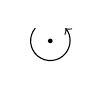
\begin{tikzpicture}
                \fill (1,1) circle (0.03);
                \draw [->] (1,1) ++(140:0.25) arc (-220:40:0.25);
            \end{tikzpicture}
            \vfill
        }
        \caption{0-cell}
    \end{subfigure}
    \begin{subfigure}[c]{0.3\textwidth}
        \centering
        \vbox to \ht\outerBox{
            \vfill
            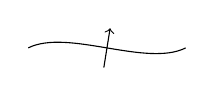
\begin{tikzpicture}
                \draw (0,1) .. controls (0.5,1.25) and (1.5,0.75) .. (2,1);
                \draw [->] (0.96,0.75) -- (1.04,1.25);
            \end{tikzpicture}
            \vfill
        }
        \caption{1-cell}
    \end{subfigure}
    \begin{subfigure}[c]{0.3\textwidth}
        \centering
        \usebox{\outerBox}
        \caption{2-cell}
    \end{subfigure}
    \caption{Outer-oriented $k$-cells in two-dimensional space.}
    \label{fig:outerExample}
\end{figure}

The distinction between inner and outer oriented $k$-cells is sensible from a physical point of view; certain physical quantities are naturally expressed in terms of inner-oriented cochains whereas other physical quantities are naturally expressed in terms of outer-oriented cochains. For example, the circulation along a line naturally resembles an inner-oriented 1-cell whereas the flux through a line naturally resembles an outer-oriented 1-cell.

\section{The Exterior Derivative}

The exterior derivative $\delta$ is used to compute derivatives, like gradients, divergences, or curls. The descrete exterior derivative is a linear map from a $(k)$-cochain to a $(k+1)$-cochain. It turns out that the standard treatment of vector calculus hides a number of important things that are applied implicitly. As shall be seen in the upcoming examples, all three of the multivariable derivatives in vector calculus (i.e. gradients, curls, and divergences) are actually one kind of derivative: the exterior derivative. The exterior derivative will be introduced by means of examples to simultaneously present some of the physical interpretations of cochains.

\subsection{Inner-Oriented Quantities}

At the end of the day we will want to know the velocity field within the domain of our problem. We will use circulation, i.e., the integral of tangential velocity along an edge, to encode velocity on the mesh in a metric free manner. Let our inner-oriented 1-cochains therefore represent circulation, defined as
\begin{flalign}
    \stepcounter{equation}
    \tag{{\theequation}a}
    & & u_{i,j} \equiv \int_L \mathbf{u} \cdot  \mathbf{\hat{t}} \, dx && \\
    \tag{{\theequation}b}
    &\text{and}& v_{i,j} \equiv \int_L \mathbf{u} \cdot \mathbf{\hat{t}} \, dy &&
\end{flalign}
where $\mathbf{\hat{t}}$ denotes the tangent vector along an edge and where the notations $u$ and $v$ are reserved for horizontal and vertical edges, respectfully. It is crucial to note that this makes circulation an integrated, not pointwise, quantity.

Figure \ref{fig:cochainExamples} shows three examples of inner-oriented $k$-cochains in two-dimensional space.

\begin{figure}[ht]
    \newsavebox\boxExample
    \savebox{\boxExample}{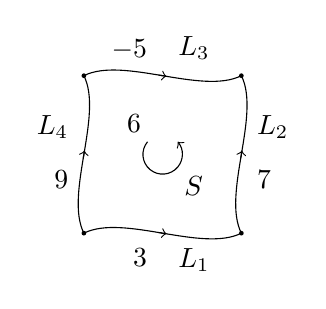
\begin{tikzpicture}
        \fill (0,0) circle (0.03) node [below left=0.5ex] at (1,0) {3} node [below right=0.5ex] at (1,0) {$L_1$};
        \fill (2,0) circle (0.03) node [below right=0.5ex] at (2,1) {7} node [above right=0.5ex] at (2,1) {$L_2$};
        \fill (2,2) circle (0.03) node [above left=0.5ex] at (1,2) {$-5$} node [above right=0.5ex] at (1,2) {$L_3$};
        \fill (0,2) circle (0.03) node [below left=0.5ex] at (0,1) {9} node [above left=0.5ex] at (0,1) {$L_4$};
        \draw (0,0) .. controls (0.5,0.25) and (1.5,-0.25) .. (2,0) .. controls (1.75,0.5) and (2.25,1.5) .. (2,2) .. controls (1.5,1.75) and (0.5,2.25) .. (0,2) .. controls (0.25,1.5) and (-0.25,0.5) .. (0,0) -- cycle;
        \draw [->] (1,1) ++(140:0.25) arc (-220:40:0.25) node [above left=1ex] at (1,1) {6} node [below right=1ex] at (1,1) {$S$};
        \draw [->] (0.95,0.008) -- (1.05,-0.008);
        \draw [->] (1.992,0.95) -- (2.008,1.05);
        \draw [->] (0.95,2.008) -- (1.05,1.992);
        \draw [->] (-0.008,0.95) -- (0.008,1.05);
    \end{tikzpicture}}
    \centering
    \begin{subfigure}[c]{0.3\textwidth}
        \centering
        \vbox to \ht\boxExample{
            \vfill
            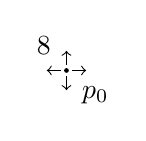
\begin{tikzpicture}
                \fill (1,1) circle (0.03) node [above left=0.5ex] {8} node [below right=0.5ex] {$p_0$};
                \draw [->] (1,1.075) -- (1,1.25);
                \draw [->] (1.075,1) -- (1.25,1);
                \draw [->] (1,0.925) -- (1,0.75);
                \draw [->] (0.925,1) -- (0.75,1);
            \end{tikzpicture}
            \vfill
        }
        \caption{0-cochain}
        \label{fig:0cochainExample}
    \end{subfigure}
    \begin{subfigure}[c]{0.3\textwidth}
        \centering
        \vbox to \ht\boxExample{
            \vfill
            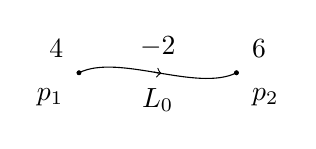
\begin{tikzpicture}
                \fill (0,1) circle (0.03) node [above left=0.5ex] {4};
                \fill (0,1) circle (0.03) node [below left=0.5ex] {$p_1$};
                \draw (0,1) .. controls (0.5,1.25) and (1.5,0.75) .. (2,1);
                \fill (2,1) circle (0.03) node [above right=0.5ex] {6};
                \fill (2,1) circle (0.03) node [below right=0.5ex] {$p_2$};
                \draw [->] (0.95,1.008) -- (1.05,0.992) node [above=0.5ex] at (1,1) {$-2$} node [below=0.5ex] at (1,1) {$L_0$};
            \end{tikzpicture}
            \vfill
        }
        \caption{1-cochain}
        \label{fig:1cochainExample}
    \end{subfigure}
    \begin{subfigure}[c]{0.3\textwidth}
        \centering
        \usebox{\boxExample}
        \caption{2-cochain}
        \label{fig:2cochainExample}
    \end{subfigure}
    \caption{Examples of $k$-cochains in two-dimensional space.}
    \label{fig:cochainExamples}
\end{figure}

Figure \ref{fig:1cochainExample} shows a 0-cochain consisting of two vertices, $p_1$ and $p_2$, and a 1-cochain composed of an edge, $L_0$. $L_0$ points from $p_1$ to $p_2$, so $p_1$ acts as a source and $p_2$ acts as a sink. Because vertices are source-like by default, as indicated in Figure \ref{fig:0cochainExample}, application of $\delta$ results in
\begin{equation}
    u = \delta(L_0) = 4 - 6 = -2
\end{equation}

Assuming that vertices represent samples of a continuous scalar field, $P$, it is clearly seen that the application of $\delta$ on a 0-cochain is analogous to the gradient operator:
\begin{equation}
    \begin{split}
        4 - 6 &= P(p_2) - P(p_1) \\
        &= \int_{L} \nabla \phi \cdot \mathbf{ds} \\
        &= \mbox{circulation}
    \end{split}
\end{equation}
The physical representation of $P$ is dynamic pressure.

Figure \ref{fig:2cochainExample} shows a 1-cochain composed of four edges and a 2-cochain composed of a single face, $S$. We apply the discrete exterior derivative by either adding or subtracting the edge values; if the orientation of a line segment opposes the orientation of the face, then its value must be subtracted. Thus, application of $\delta$ on $S$ results in
\begin{equation}
    \xi = \delta(S) = 3 + 7 - (-5) - 9 = 6
\end{equation}

Application of $\delta$ on a 1-cochain is analogous to the curl operator because
\begin{equation}
    \begin{split}
        3 + 7 - (-5) - 9 &= u_1(L_1) + v_2(L_2) - u_2(L_3) - v_1(L_4) \\
        &= \int_{L_1} \mathbf{u} \cdot \mathbf{dl} + \int_{L_2} \mathbf{u} \cdot \mathbf{dl} - \int_{L_3} \mathbf{u} \cdot \mathbf{dl} - \int_{L_4} \mathbf{u} \cdot \mathbf{dl} \\
        &= \oint_{\partial S} \mathbf{u} \cdot \mathbf{dl} \\
        &= \iint_{S} \left( \nabla \times \mathbf{u} \right) \cdot dA
    \end{split}
    \label{eq:curlExample}
\end{equation}
where $\partial S \equiv L_1 \cup L_2 \cup L_3 \cup L_4$. This is not the only insight to be gained here; recall that the circulation along a closed contour, denoted $\Gamma$, is defined as:
\begin{equation}
    \Gamma \equiv \oint_C \mathbf{u} \cdot \mathbf{dl}
    \label{eq:circulation}
\end{equation}
Comparing Equations \eqref{eq:curlExample} and \eqref{eq:circulation}, we conclude that the $\delta(S)$ must represent the circulation around the edges of $S$. Circulation is related to vorticity; the circulation around a closed contour is equal to the integrated vorticity enclosed by that contour. From Stokes' theorem:
\begin{equation}
    \Gamma \equiv \oint_C \mathbf{u} \cdot \mathbf{dl} = \iint_A \left( \nabla \times \mathbf{u} \right) dA = \iint_A \xi \; dA
\end{equation}
Therefore, if the area of $S$ is infinitesimal, then $\xi$ represents vorticity.

Because $3$-cochains are undefined in two-dimensional space, the application of $\delta$ on a 2-cochain results in the empty set by definition. In a similar vein, 0-cochains can only be the result of the application of $\delta$ on a real number.

\subsection{Outer-Oriented Quantities}

We use flux, i.e., the integral of the normal velocity along an edge, as a metric free representation of velocity on an outer-oriented mesh. Note again that this makes flux an integrated, not pointwise, quantity. Thus, let the outer-oriented 1-cochains represent flux, defined as
\begin{flalign}
    \stepcounter{equation}
    \tag{{\theequation}a}
    & & \tilde{u}_{i,j} \equiv \int_L \mathbf{u} \cdot  \mathbf{\hat{n}} \, dy && \\
    \tag{{\theequation}b}
    &\text{and}& \tilde{v}_{i,j} \equiv \int_L \mathbf{u} \cdot \mathbf{\hat{n}} \, dx &&
\end{flalign}
where $\mathbf{\hat{n}}$ denotes the normal vector along the line segment and where $u_{i,j}$ and $v_{i,j}$ are again reserved for horizontal and vertical edges, respectively.
Figure \ref{fig:outerCochainExamples} shows three examples of outer-oriented $k$-cochains in two-dimensional space.

\begin{figure}[ht]
    \newsavebox\boxOuterExample
    \savebox{\boxOuterExample}{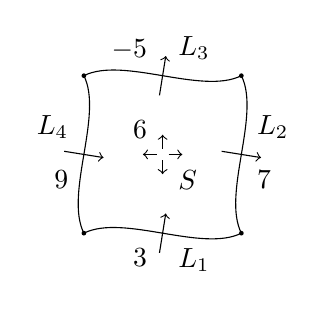
\begin{tikzpicture}
        \fill (0,0) circle (0.03) node [below left=0.5ex] at (1,0) {3} node [below right=0.5ex] at (1,0) {$L_1$};
        \fill (2,0) circle (0.03) node [below right=0.5ex] at (2,1) {7} node [above right=0.5ex] at (2,1) {$L_2$};
        \fill (2,2) circle (0.03) node [above left=0.5ex] at (1,2) {$-5$} node [above right=0.5ex] at (1,2) {$L_3$};
        \fill (0,2) circle (0.03) node [below left=0.5ex] at (0,1) {9} node [above left=0.5ex] at (0,1) {$L_4$};
        \draw (0,0) .. controls (0.5,0.25) and (1.5,-0.25) .. (2,0) .. controls (1.75,0.5) and (2.25,1.5) .. (2,2) .. controls (1.5,1.75) and (0.5,2.25) .. (0,2) .. controls (0.25,1.5) and (-0.25,0.5) .. (0,0) -- cycle;
        \node [above left=0.5ex] at (1,1) {6};
        \node [below right=0.5ex] at (1,1) {$S$};
        \draw [->] (0.96,-0.25) -- (1.04,0.25);
        \draw [->] (1.75,1.04) -- (2.25,0.96);
        \draw [->] (0.96,1.75) -- (1.04,2.25);
        \draw [->] (-0.25,1.04) -- (0.25,0.96);
        \draw [->] (1,1.075) -- (1,1.25);
        \draw [->] (1.075,1) -- (1.25,1);
        \draw [->] (1,0.925) -- (1,0.75);
        \draw [->] (0.925,1) -- (0.75,1);
    \end{tikzpicture}}
    \centering
    \begin{subfigure}[c]{0.3\textwidth}
        \centering
        \vbox to \ht\boxOuterExample{
            \vfill
            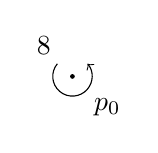
\begin{tikzpicture}
                \fill (1,1) circle (0.03) node [above left=1ex] {8} node [below right=1ex] {$p_0$};
                \draw [->] (1,1) ++(140:0.25) arc (-220:40:0.25);
            \end{tikzpicture}
            \vfill
        }
        \caption{0-cochain}
        \label{fig:outer0CochainExample}
    \end{subfigure}
    \begin{subfigure}[c]{0.3\textwidth}
        \centering
        \vbox to \ht\boxOuterExample{
            \vfill
            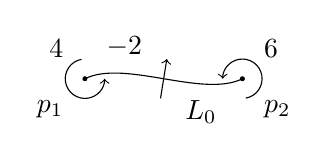
\begin{tikzpicture}
                \draw [->] (0,1) ++(100:0.25) arc (-260:0:0.25);
                \draw [->] (2,1) ++(280:0.25) arc (-80:180:0.25);
                \fill (0,1) circle (0.03) node [above left=1ex] {4};
                \fill (0,1) circle (0.03) node [below left=1ex] {$p_1$};
                \draw (0,1) .. controls (0.5,1.25) and (1.5,0.75) .. (2,1);
                \fill (2,1) circle (0.03) node [above right=1ex] {6};
                \fill (2,1) circle (0.03) node [below right=1ex] {$p_2$};
                \draw [->] (0.96,0.75) -- (1.04,1.25) node [above left=1ex] at (1,1) {$-2$} node [below right=1ex] at (1,1) {$L_0$};
            \end{tikzpicture}
            \vfill
        }
        \caption{1-cochain}
        \label{fig:outer1CochainExample}
    \end{subfigure}
    \begin{subfigure}[c]{0.3\textwidth}
        \centering
        \usebox{\boxOuterExample}
        \caption{2-cochain}
        \label{fig:outer2CochainExample}
    \end{subfigure}
    \caption{Examples of $k$-cochains in two-dimensional space.}
    \label{fig:outerCochainExamples}
\end{figure}

Figure \ref{fig:outer1CochainExample} shows a 0-cochain composed of two vertices, $p_1$ and $p_2$, and a 1-cochain composed of an edge, $L_0$. The recipe for applying $\delta$ is straightforward: add those values at vertices that share a common orientation with the edge and subtract those values whose orientation opposes the orientation of the edge. The orientation of $p_2$, for example, opposes the orientation of $L_0$ because the arrows point in opposite directions. Thus,
\begin{equation}
    \tilde{u} = \delta(L_0) = 4 - 6 = -2
\end{equation}
This procedure is analogous to the gradient operator because
\begin{equation}
    \begin{split}
        4 - 6 &= \psi(p_2) - \psi(p_1) \\
        &= \int_{L} \nabla \psi \cdot \mathbf{ds} \\
        &= \mbox{flux}
    \end{split}
\end{equation}

What do the values at the vertices, $\psi$, physically represent? If edges represent flux, then vertices must represent the stream function, $\psi$. Here is why: the numerical value of $\psi$ is defined such that the difference $\Delta \psi$ between two streamlines is equal to the mass flux between the two streamlines. This fact allows us to determine the stream function up to a constant.

Figure \ref{fig:outer2CochainExample} shows an outer-oriented 1-cochain composed of four edges and an outer-oriented 2-cochain composed of a plane, $S$. The plane is source-like as indicated by the outward pointing arrows. That is, an outflow is defined positive. We apply the discrete exterior derivative by adding flows into the plane and subtracting flows out of the plane. Thus, application of $\delta$ results in
\begin{equation}
    \tilde{\xi} = \delta(S) = -3 + 7 - 5 - 9 = -10
\end{equation}

Application of $\delta$ on a 1-cochain is analogous to the curl operator because
\begin{equation}
    \begin{split}
        -3 + 7 + (-5) - 9 &= -\tilde{u}_1(L_1) + \tilde{v}_2(L_2) + \tilde{u}_2(L_3) - \tilde{v}_1(L_4) \\
        &= -\int_{L_1} \mathbf{u} \cdot \mathbf{dl} + \int_{L_2} \mathbf{u} \cdot \mathbf{dl} + \int_{L_3} \mathbf{u} \cdot \mathbf{dl} - \int_{L_4} \mathbf{u} \cdot \mathbf{dl} \\
        &= \oint_{\partial S} \mathbf{u} \cdot \mathbf{dl} \\
        &= \iint_{S} \left( \nabla \times \mathbf{u} \right) \cdot dA
    \end{split}
    \label{eq:curlExample}
\end{equation}
where $\partial S \equiv L_1 \cup L_2 \cup L_3 \cup L_4$. 

What is the physical representation of $\tilde{\xi}$? The fluid is incompressible, so the velocity field must be divergence free (i.e., $\nabla \cdot \mathbf{u} = 0$). According to the generalized Stokes' theorem the integral of the divergence over a plane equals the sum of the fluxes on all four edges. In other words, everything that gets in must also get out. The 2-cell $\tilde{\xi}$ therefore represents the rate of mass production in the plane. Thus, for the law of mass conservation to hold true, $\tilde{\xi}$ must be equal to zero in each and every plane.

\subsection{DeRham Complex}

The results of this section can be summarized in a diagram called the DeRham complex:
\begin{equation}
    \begin{gathered}
        \xymatrix@C=13ex{
            \mathbb{R} \ar[r]^{\delta} & C^{(0)} \ar[r]^{\delta}_{\text{grad}} & C^{(1)} \ar[r]^{\delta}_{\text{curl}} & C^{(2)} \ar[r]^{\delta} & \emptyset \\
            \mathbb{R} \ar[r]^{\delta} & \tilde{C}^{(0)} \ar[r]^{\delta}_{\text{grad}} & \tilde{C}^{(1)} \ar[r]^{\delta}_{\text{curl}} & \tilde{C}^{(2)} \ar[r]^{\delta} & \emptyset
        }
    \end{gathered}
\end{equation}

A major advantage of the discrete exterior derivative is that it satisfies the same rules and identities as its smooth counterpart. The discrete exterior derivative is mathematically exact because it acts on and produces integrated quantities. That is, application of $\delta$ does not introduce any error whatsoever. As we shall see, this property contributes to the strength of DEC as a whole and it results in preservation of the physics implied in the smooth governing equations.

\section{The Hodge-$\star$ Operator}

We have established that two-dimensional space supports points, lines, and planes. Let us briefly digress to three-dimensional space for the sake of familiarity; three-dimensional space supports points, lines, planes, and volumes. In three-dimensional space, we can have one linearly independent volume, three linearly independent planes, and three linearly independent lines. It is a bit awkward to think of linearly independent points, but there is just one linearly independent point in three-dimensional space. This 1--3--3--1 sequence suggests a pairing; there exists a vector space isomorphism between $k$-vectors and $(n-k)$-vectors. The Hodge-$\star$ operator is a linear map between inner-oriented $k$-cochains and outer-oriented $(n-k)$-cochains or vice versa, where $n$ denotes the dimension of the vector space.

We have introduced the $\delta$ operator to map $(k)$-cochains to $(k+1)$-cochains. However, the Navier-Stokes equations equate both inner and outer oriented cochains, which requires the Hodge-$\star$ operator. The Hodge-$\star$ operator links the DeRham complexes for inner and outer oriented cochains. This linked structure is called the double DeRham complex:
\begin{equation}
    \begin{gathered}
        \xymatrix@=13ex{
            \mathbb{R} \ar[r]^{\delta} & C^{(0)} \ar[r]^{\delta}_{\text{grad}} \ar@{<->}[d]^{\star} & C^{(1)} \ar[r]^{\delta}_{\text{curl}} \ar@{<->}[d]^{\star} & C^{(2)} \ar@{<->}[d]^{\star} \ar[r]^{\delta} & \emptyset \\
            \emptyset & \tilde{C}^{(2)} \ar[l]_{\delta} & \tilde{C}^{(1)} \ar[l]_{\delta}^{\text{curl}} & \tilde{C}^{(0)} \ar[l]_{\delta}^{\text{grad}} & \mathbb{R} \ar[l]_{\delta}
        }
    \end{gathered}
    \label{eq:doubleDeRham}
\end{equation}

In a discrete setting, cochains are stored in vectors, $\delta$ operators are represented by incidence matrices, $\mathbb{E}$, and Hodge-$\star$ operators are represented by Hodge matrices, $\mathbb{H}$. In such a framework, application of the $\delta$ or Hodge-$\star$ operator becomes a matrix vector-multiplication. Hence, the double DeRham complex in Equation \eqref{eq:doubleDeRham} becomes
\begin{equation}
    \begin{gathered}
        \xymatrix@=13ex{
            C^{(0)} \ar[r]^{\mathbb{E}^{(1,0)}}_{\text{grad}} \ar@<1ex>[d]^{\mathbb{H}^{(\tilde{2},0)}} & C^{(1)} \ar[r]^{\mathbb{E}^{(2,1)}}_{\text{curl}} \ar@<1ex>[d]^{\mathbb{H}^{(\tilde{1},1)}} & C^{(2)} \ar@<1ex>[d]^{\mathbb{H}^{(\tilde{0},2)}} \\
            \tilde{C}^{(2)} \ar@<1ex>[u]^{\mathbb{H}^{(0,\tilde{2})}} & \tilde{C}^{(1)} \ar[l]_{\tilde{\mathbb{E}}^{(2, 1)}}^{\text{curl}} \ar@<1ex>[u]^{\mathbb{H}^{(1,\tilde{1})}} & \tilde{C}^{(0)} \ar[l]_{\tilde{\mathbb{E}}^{(1,0)}}^{\text{grad}} \ar@<1ex>[u]^{\mathbb{H}^{(2,\tilde{0})}}
        }
    \end{gathered}
\end{equation}
